\subsubsection{Configure GBTx DB to use external \itwoc adapter}
\label{sec:hardware-ext-i2c}
This setup is required to program a GBTx DB using an external \itwoc adapter.
Follow \autoref{fig:external_i2c} to connect an external \itwoc
adapter\footnote{
    In UMD lab, on the USB \itwoc adapter, the color coding is:
    yellow $\rightarrow$ \texttt{I2C SCL};
    blue $\rightarrow$ \texttt{I2C SDA};
}.

\begin{figure}[!ht]
\centering
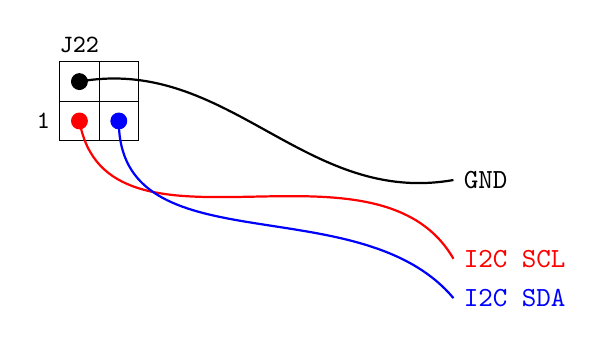
\begin{tikzpicture}
    % Pins
    \draw (0,0) rectangle (0.5,0.5);
    \draw (0.5,0) rectangle (1,0.5);
    \draw (0,-0.5) rectangle (0.5,0);
    \draw (0.5,-0.5) rectangle (1,0);

    % PCB labels
    \coordinate (A) at (0.25,0.5);
    \node at (A) [above] {\small\texttt{J22}};
    \coordinate (B) at (0,-0.25);
    \node at (B) [left] {\small\texttt{1}};

    % GND
    \draw [black,fill] (0.25,0.25) circle [radius=0.1];
    \draw [thick] (0.25,0.25)
        to [out=10,in=190] (5,-1) node [right] {\texttt{GND}};

    % I2C SCL
    \draw [red,fill] (0.25,-0.25) circle [radius=0.1];
    \draw [red,thick] (0.25,-0.25) to [out=-80,in=120] (5,-2)
        node [right] {\texttt{I2C SCL}};

    % I2C SDA
    \draw [blue,fill] (0.75,-0.25) circle [radius=0.1];
    \draw [blue,thick] (0.75,-0.25) to [out=-90,in=130] (5,-2.5)
        node [right] {\texttt{I2C SDA}};
\end{tikzpicture}
\caption{Schematic for external \itwoc adapter setup.}
\label{fig:external_i2c}
\end{figure}
